\section{Source Code Management}
\label{sec:scm}

\ac{SCM}\index{source code management} or in similar context also called \ac{VCS}\index{version control system} is a system that records changes to a file or set of files over time so that you can recall specific versions later.~\autocite{Chacon:2014:ProGit:27}
\ac{VCS} can be used for/with nearly any type of file on a computer, apart from is it a source code of program or not.
With this tool, we can historically track each changes of our files.
Sometimes very needed when we want to revert back the files or even an entire repository to the previous state we mistakenly edit, also redo it back to future state.
More features also include comparing difference in changes, see who created or modified what, and most of all is enable an easier way to collaborate with more than one person.
The specific style of \ac{VCS} we're using is a \ac{DVCS}.
\ac{DVCS} enables full mirror of the repository, so there is an indepentent access and modification for each in server or local repository, illustrated as such in \autoref{fig:dvcs}.

\begin{figure}[htb]
    \centering
    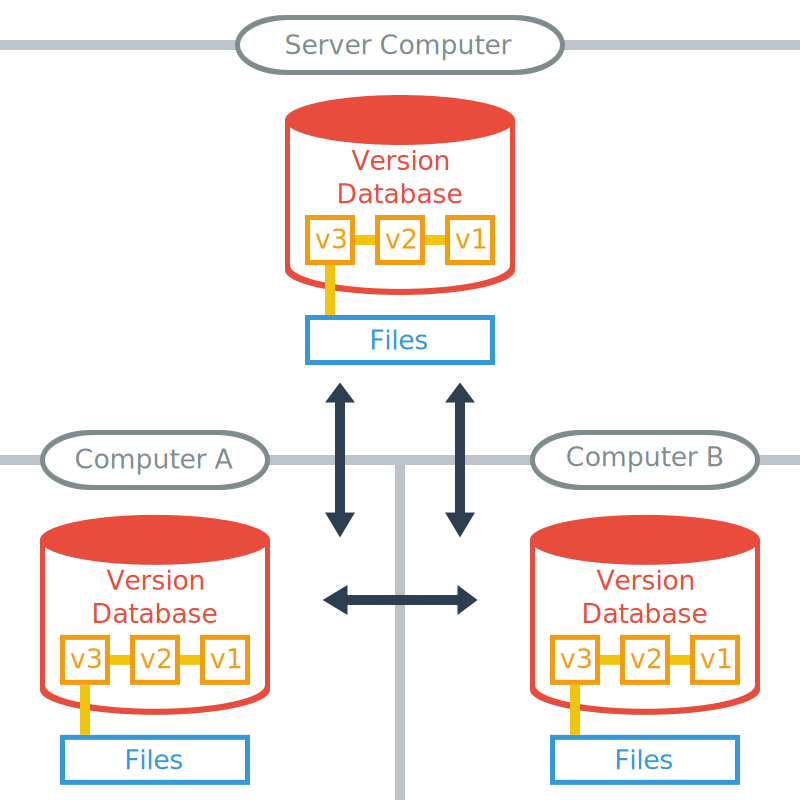
\includegraphics[height=7cm]{\dir/include/dvcs.png}
    \caption[DVCS illustrated]{DVCS illustrated}
    \label{fig:dvcs}
\end{figure}

% --------------------------------------------------
\subsection{Git}

\begin{wrapfigure}{r}{0.5\textwidth}
  \vspace{-20pt}
  \begin{center}
    \includegraphics[width=4.5cm]{\dir/include/logo/git.png}
  \end{center}
  \vspace{-20pt}
  \caption{Git logo}
  \label{fig:git-logo}
  \vspace{-10pt}
\end{wrapfigure}

Git is more than a \ac{VCS}, it is a \ac{DVCS} which takes a decentralized way of managing a repository.
It is a free and open source distributed version control system designed to handle everything from small to very large projects with speed and efficiency.~\autocite{Git2010}
In \autoref{fig:git-stages}, we can see how Git stages works at a glance.
Basically we work in the working directory, then we add the changed files into the staging area, once it has been confirmed, those changes committed into the Git repository.
It works more effectively because the stage called ``staging area'' or ``index'' enables that commits can be reviewed before actually completing the commit~\autocite{Git2010}.

\begin{figure}[htb]
    \centering
    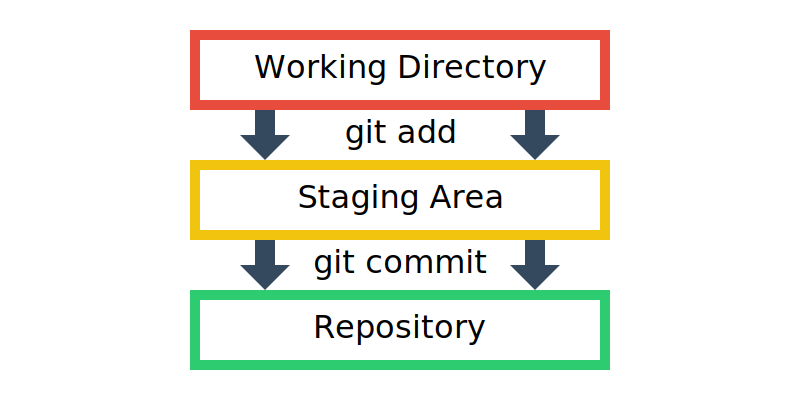
\includegraphics[width=6cm]{\dir/include/git-stages.png}
    \caption{Git stages}
    \label{fig:git-stages}
\end{figure}

% --------------------------------------------------
\subsection{GitHub}

\begin{wrapfigure}{r}{0.5\textwidth}
  \vspace{-20pt}
  \begin{center}
    \includegraphics[width=4.5cm]{\dir/include/logo/github.png}
  \end{center}
  \vspace{-20pt}
  \caption{GitHub logo}
  \label{fig:github-logo}
  \vspace{-10pt}
\end{wrapfigure}

In order to distribute and help a better colloaboration with Git, we use a Git hosting service called GitHub.
GitHub is a web-based service for Git repositories that offers \ac{DVCS} and \ac{SCM} features, also combined with various useful features like issue tracking and code review.
As they declared, GitHub is the best place to share code with friends, co-workers, classmates, and complete strangers~\autocite{GitHub2015}.
It is one of the most used collaboration tool for a lot of developers and projects.
Many open-source projects are using it and hosted in it.
Other alternatives available that presented as a web service are BitBucket, Assembla, and Kiln.
In general, those are places where everyone can share their source code files and even stories with the world.
